\section{Model}
\label{sec:shapes}
\begin{figure*}[!t]
\centering
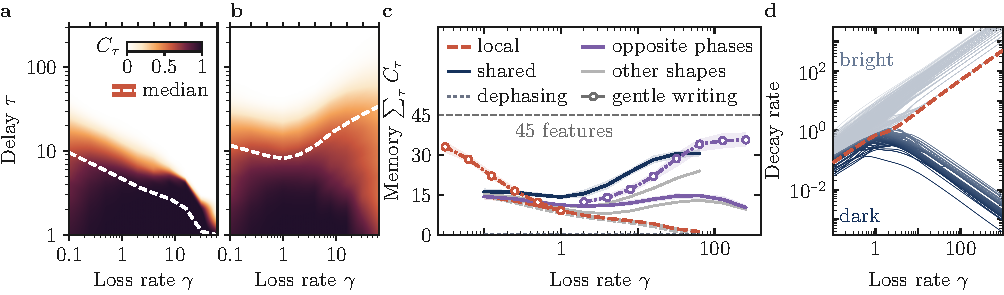
\includegraphics[width=\textwidth]{figures/fig2_clock.pdf}
\caption{\textbf{The decay structure decides whether loss shortens or prolongs the memory.}
\textbf{a,b}~Recall of the input $\tau$ steps back (colour) against the loss rate, for independent decay (a) and the
equal-phase channel (b). The dashed line marks the median delay, which splits the recall in half.
\textbf{c}~Linear memory capacity at the full input strength and with gentle writing, an input that weakens as the
memory lifetime grows (Sec.~\ref{sec:writing}).
\textbf{d}~All decay rates with the equal-phase channel: the dark modes slow down as the loss grows, while the slowest
mode of independent decay (dashed) speeds up.}
\label{fig:clock}
\end{figure*}

The reservoir is the driven spin system of Ref.~\cite{Sannia2024}. Five spins ($N=5$) interact through random
couplings $J_{ij}$, and in each step a random input $u$ between 0 and 1 sets the strength of a transverse field for a
time $\Delta t$:
\begin{equation}
  H(u)=\sum_{i<j}J_{ij}X_iX_j+h\sum_iZ_i+h(1+u)\sum_iX_i ,
  \label{eq:H}
\end{equation}
with Pauli operators $X_i$, $Z_i$ of spin $i$ and a field strength $h$. To weaken the input at a fixed mean drive, we
replace $h(1+u)$ by $h[\tfrac32+\eta(u-\tfrac12)]$, where the amplitude $\eta$ scales how far each input moves the
field. The state $\rho$ of the spins follows a Lindblad master
equation~\cite{Gorini1976,Lindblad1976},
\begin{equation}
  \dot\rho=-i[H(u),\rho]+\sum_k\Bigl(L_k\rho L_k^\dagger-\tfrac12\{L_k^\dagger L_k,\rho\}\Bigr),
  \label{eq:lindblad}
\end{equation}
where the Hamiltonian drives the internal dynamics and each jump operator $L_k$, scaled by one loss rate $\gamma$, is
one way the environment changes the state, such as removing an excitation or erasing a phase.

A linear readout of 45 features, the single-spin and two-spin expectation values, is trained to estimate the input
from $\tau$ steps back. Its recall $C_\tau$, between 0 and 1, is the squared correlation between the estimate and the
input on held-out data. The linear memory capacity $\sum_\tau C_\tau$ adds up the recall over all delays. One unit is
one past input recalled perfectly, and the ceiling is 45, the number of features. The memory lifetime
$t_{\mathrm{mem}}$ says how long the variance of a stored signal survives, and the single-input recall time
$t_{\mathrm f}$ how long one input stays linearly readable on its own (Appendices~\ref{sec:methods-slow} and~\ref{sec:order}). Sections~\ref{sec:clock}
to~\ref{sec:writing} use exact expectation values, as if every measurement were repeated infinitely often, and
Sec.~\ref{sec:price} counts measurements.

We compare decay channels at equal total coupling $\Tr K=\sum_k\Tr L_k^\dagger L_k$ and hold the Hamiltonian fixed
to isolate the effect of the dissipative structure. The generator of Eq.~\eqref{eq:lindblad} has $4^N$ modes,
patterns of change in the state that each decay at their own rate. Equal total coupling fixes their mean rate for
every Hamiltonian, but not the slow modes, which keep a record longest and can become slower or faster
(Appendix~\ref{sec:methods-shapes}). Table~\ref{tab:families} lists the eight channels we studied.

Four of them carry the argument (Fig.~\ref{fig:concept}b). With independent decay every spin loses its excitation on
its own. With collective decay all spins lose it through one shared channel, either with equal phases or with
opposite phases on spins 4 and 5. We call these the equal-phase and the opposite-phase channel. With dephasing every
spin loses its phase. What tells them apart is whether the dissipation leaves only a single stationary state or a
protected subspace that can carry a record. Operators that the dissipation alone leaves unchanged are
protected, although the Hamiltonian can still turn them or couple them to decaying ones. Independent decay protects only
its ground state. Neither collective channel can empty its ten dark states, so every operator on them is protected.
Dephasing keeps the populations, the probabilities of the spin configurations, but erases the coherences between
them. Every step then leaves the fully mixed state, with equal populations and no coherence, unchanged whatever the
input: the dynamics is unital. The driven reservoir relaxes to this state, after which no input leaves a trace, so
dephasing stores nothing.

\section{Results}
\label{sec:results}

\subsection{Dissipative structure controls memory lifetime}
\label{sec:clock}
Increasing the loss separates the channels into distinct memory regimes (Fig.~\ref{fig:clock}). With independent decay, recall retreats to ever shorter delays and the linear memory capacity
falls steadily (Fig.~\ref{fig:clock}a,c). With the equal-phase channel the capacity first dips and then doubles, and
at strong loss inputs fifty steps back are still recalled (Fig.~\ref{fig:clock}b,c). The other channels split the same
way (Fig.~\ref{fig:clock}c, grey): exchange and gain/loss follow independent decay, two collective channels follow the
equal-phase channel, and pairwise decay follows the opposite-phase channel. The decay rates show the split
(Fig.~\ref{fig:clock}d). Without protected operators the slowest rate grows in proportion to $\gamma$ and the memory
lifetime shrinks. With dark states the slow rates fall as $1/\gamma$ and the lifetime grows.

Why does stronger collective decay prolong the memory? In the two-spin picture of Fig.~\ref{fig:concept}c, the dark
state $|{-}\rangle\propto|10\rangle-|01\rangle$ can decay only through the bright state
$|{+}\rangle\propto|10\rangle+|01\rangle$, and the Zeno effect~\cite{Beige2000,FacchiPascazio2002} suppresses this
escape. Its rate falls as $\Omega^2/\gamma$, where $\Omega$ couples $|{+}\rangle$ and $|{-}\rangle$, just as the slow
mode of an overdamped oscillator settles more slowly the stronger the friction.

This protection follows from the strong-loss expansion at fixed system size. At strong loss the reservoir follows its Hamiltonian restricted to the dark
states, which turns the stored state but cannot make it decay. Decay enters only at the next order, when the
Hamiltonian briefly lifts a dark state into a bright one~\cite{Zanardi2014,Reiter2012}. One step is then a rotation
plus a loss that falls as $1/\gamma$ (Eq.~\eqref{eq:reduced}): a nearly orthogonal map with a small but finite decay rate, the
classic recipe for a long memory in a network~\cite{White2004}. Calculations for three to six spins show the same decay out of the dark states, falling as $1/\gamma$ with
different prefactors (Appendix~\ref{app:num-lifetime}).

Two tests show that the dark states hold the memory (Appendix~\ref{app:num-lifetime}). A model of the ten dark states
alone, with no fitted parameter, reproduces the recall of the full reservoir at strong loss. Replacing the protected
components of the state by their time averages after every step, which removes their dependence on the inputs,
destroys all memory beyond a few steps, while the same operation on a randomly rotated set of equal size leaves most
of it. Residual local noise caps this lifetime: for the
equal-phase channel, our estimate requires a ratio of collective to local loss rates that grows quadratically with the
target recall time (Appendix~\ref{app:num-noise}).

Dark states thus protect stored information against decay. With the opposite-phase channel, however, the dark states
are just as protected, yet the capacity returns only to its weak-loss level (Fig.~\ref{fig:clock}c). The reason is
the ongoing input.

\subsection{New inputs mix stored information}
\label{sec:mixing}
Each new input turns the stored state slightly, by an angle that depends on the input (Fig.~\ref{fig:concept}d), so to an old input every newer input acts as noise. Over the
memory lifetime the stored direction takes a random walk of small turns $\pm\theta$ and spreads by about
$\theta\sqrt{t_{\mathrm{mem}}}$. Once the spread reaches about a radian, the record of an old input survives only
multiplied by the inputs that followed it, and a linear readout cannot turn such products back into single inputs.

A stored contribution can therefore depend on one past input or on several jointly. We count the distinct past inputs
that it depends on and call this number $D$. A function of $u_{t-3}$ alone has $D=1$, even if it is nonlinear in
$u_{t-3}$, and $u_{t-3}u_{t-5}$ has $D=2$. The information processing
capacity~\cite{Dambre2012,MartinezPenaIPC2023} also counts how well the readout reconstructs nonlinear functions of
past inputs, and sorting its contributions by $D$ separates information about single inputs from information about
several jointly (Appendix~\ref{sec:order}). The
disturbance caused by one input is measured by its mixing fraction $s$, between 0 and 1: the part of a stored signal
that one input turns differently from the average input. For small turns it grows as the square of the turn. The law
concerns the covariance of the state, how its components fluctuate together across input histories, and assumes that
one pattern of these fluctuations, a single slow direction of the covariance, outlives all others, even when many
slow components of the state share it. Our main theorem then says that a stored contribution
involves on average $s\,t_{\mathrm{mem}}$ inputs, the disturbance per input times the memory lifetime:

\begin{keybox}
\begin{theorem}[Mixing law, made precise in Appendix~\ref{app:law}]\label{thm:law}
Let a reservoir be reset with probability $p$ per step, so that $t_{\mathrm{mem}}\sim1/(2p)$ as $p\to0$, and otherwise turned by
input-dependent unitaries that mix the stored state, leave a single slow direction of the stored covariance, and
write a signal (conditions in Appendix~\ref{app:law}). Pick a stored contribution with probability equal to its share
of the capacity, and let $D$ be the number of distinct inputs it depends on. As $p\to0$, $D/t_{\mathrm{mem}}$ becomes
exponentially distributed with mean $s$, and
\begin{equation*}
  \mathbb ED=s\,t_{\mathrm{mem}}+O(1).
\end{equation*}
\end{theorem}
\end{keybox}
\begin{figure*}[!t]
\centering
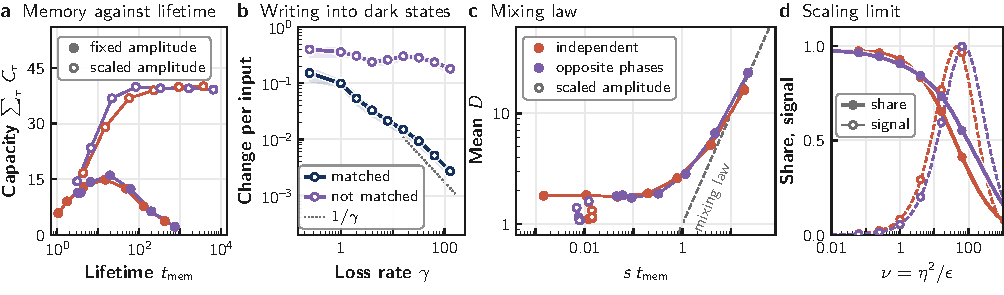
\includegraphics[width=\textwidth]{figures/fig3_price.pdf}
\caption{\textbf{New inputs mix stored information, and gentle writing limits the mixing.}
\textbf{a}~Single-input recall time for four input amplitudes $\eta$, rescaled as the sum of decay and mixing
predicts: for each channel all amplitudes fall on one curve.
\textbf{b}~How strongly one input writes into the dark states of the equal-phase channel: an input aligned with the
channel, the same on every spin, fades as $1/\gamma$, while a pattern that sums to zero over the spins keeps writing.
\textbf{c}~Mean number $D$ of inputs mixed into a stored contribution of the five-spin reservoir, against the mixing
law: at the full input strength it follows $s\,t_{\mathrm{mem}}$, and gentle writing keeps it near one.
\textbf{d}~One qubit, turned by $\theta$ per input and relaxing at the rate $\epsilon$: the stored signal (solid,
relative to its maximum) peaks at an intermediate $\theta^2/\epsilon$, the squared turn accumulated over one relaxation
time (dotted), where single inputs (dashed) still carry 80\% of the capacity.}
\label{fig:mixing}
\end{figure*}


The reason is a race: in each step a fraction $s$ of the stored signal picks up one more input, while a fraction
$1/t_{\mathrm{mem}}$ of it is lost, so the number of inputs follows a geometric distribution, which becomes exponential
for long memories. The same covariance condition extends the law to physical channels without a reset, with the slow decay in place
of the reset (Appendix~\ref{app:physical}), while several slow covariance directions keep distinct mixing scales
(Appendix~\ref{app:slowdir}). Nothing in the law is quantum: classical state-affine reservoirs, whose state is updated
by an input-dependent linear map plus an offset~\cite{GrigoryevaOrtegaSAS2018}, obey it under the same conditions. Dissipation enters through its two factors, the memory lifetime and the disturbance per input.

Exact covariance calculations, Eq.~\eqref{eq:recursion}, support the law in the five-spin reservoir
(Fig.~\ref{fig:mixing}c). At the full input amplitude one input disturbs the stored state only slightly, $s\approx0.02$, and the
mean of $D$ grows with the memory lifetime as $s\,t_{\mathrm{mem}}$ plus an offset of one to two inputs, as
Theorem~\ref{thm:law} allows (Appendix~\ref{app:num-capacity}). At a fixed input strength, a longer memory is
therefore a more mixed one. How must the input strength change with the memory lifetime so that individual
inputs remain readable?

\subsection{Matching input strength to memory lifetime}
\label{sec:writing}
The mixing law suggests weakening each new input as the memory lifetime grows. Because the disturbance $s$ grows as
the square of the turn, keeping $s\,t_{\mathrm{mem}}$ fixed requires an input amplitude proportional to
$1/\sqrt{t_{\mathrm{mem}}}$. We call this gentle writing. A gentler input would write too little: one qubit makes the
trade-off exact (Fig.~\ref{fig:mixing}d, Appendix~\ref{app:qubit}). Its stored signal is largest when the squared turn
per input, accumulated over one relaxation time, is of order one, and only a turn that falls as
$1/\sqrt{t_{\mathrm{mem}}}$ keeps the signal finite as the memory grows.

The single-input recall time shows the same balance. Its rate adds the decay of the stored signal and a mixing rate
that grows as $\eta^2$ (Appendix~\ref{sec:methods-slow}). The decay grows as $\gamma$ with
independent decay and falls as $1/\gamma$ with the opposite-phase channel, so $\eta^2t_{\mathrm f}$ should depend on
loss and input only through $\gamma/\eta^2$ and through $\gamma\eta^2$, respectively. Both collapses hold for four
input amplitudes (Fig.~\ref{fig:mixing}a).

Gentle writing more than doubles the linear memory capacity. In the five-spin reservoir the amplitude falls as
$1/\sqrt\gamma$ for the opposite-phase channel, whose lifetime grows with the loss, and as $\sqrt\gamma$ for independent
decay, whose lifetime grows as the loss weakens (Fig.~\ref{fig:clock}c, circles). With exact readout the capacity rises
from about 15 to 35 units for both channels (Table~\ref{tab:memory}). Since the capacities of all orders add up to the 45
features~\cite{Dambre2012}, the gain moves capacity from combinations of inputs to individual inputs. A
long memory therefore needs no dark states: weak independent decay with gentle writing reaches one too. What dark
states add is a memory that stays long under strong dissipation and grows with the loss.

The phases of the collective channel decide whether an input reaches the protected memory at all. Spin $i$ couples to
the shared channel with the sign $c_i=\pm1$, and the dark states are annihilated by the collective lowering operator
$\sum_ic_i\sigma_i^-$. We call an input field aligned with the channel if its strength on each spin is proportional to
$c_i$. An aligned field $\sum_ic_iX_i$ is the lowering operator plus its adjoint, so it cannot couple two dark states.
It writes into them only through brief excursions into bright states, with a strength that falls as $1/\gamma$, while
the non-aligned part of any other field writes into them directly (Fig.~\ref{fig:mixing}b,
Appendix~\ref{app:num-mixing}). The uniform input of Eq.~\eqref{eq:H} is aligned with the equal-phase channel, so it
writes gently by itself, and this channel comes close to the gain of gentle writing at the full amplitude. With the
opposite-phase channel it is not aligned and must be weakened. This automatic gentle writing relies on exact
alignment: a phase error opens a direct coupling within the dark subspace (Appendix~\ref{app:num-mixing}).

For three spins with the opposite-phase channel we prove both regimes (Appendix~\ref{app:spins}). At a fixed amplitude
single inputs lose their share of the capacity, while with an amplitude $\eta_0/\sqrt\gamma$ they keep it and are
recalled ever further back. The record is written into coherences between the energy levels of the Hamiltonian
restricted to the dark states. Coherence shapes the
performance of spin reservoirs~\cite{Palacios2024}, and erasing these coherences after every input collapses the
stored signal as $1/\gamma^2$. A gentler input, however, writes a fainter record. With exact readout this costs
nothing. With measurements it does.

\subsection{Measurement limits recoverable memory}
\label{sec:price}
Exact expectation values remove the cost of resolving weak signals. A memory whose input strength is matched to its
lifetime grows longer, not larger: it cannot exceed the 45 features, so each delay is recalled more faintly.

For projective readout, each feature is estimated from repeated preparations of the reservoir. Each preparation
replays a finite window of inputs, which grows with the memory lifetime, before it is measured~\cite{Cindrak2024}. We
therefore count the budget in reservoir steps, preparations times replayed steps summed over the measurement settings,
per output step, and simulate the replay (Appendix~\ref{sec:methods-sampling}).

Under this projective-readout protocol, weak independent decay with gentle writing recovers the most memory at a fixed
budget (Fig.~\ref{fig:sampling}a). At a budget of $10^9$ reservoir steps per output step it keeps 34 units, nearly all
of its exact capacity, against 21 for the opposite-phase channel at its best sampled loss rate near $\gamma=64$. The
dark-state memory lasts as long as that of weak independent decay, but its signal is about three times fainter. The
equal-phase channel, whose exact capacity grows with the loss, now loses capacity as the loss grows.

The size of the signal is set by the state that the dissipation leaves behind. An input acts on the stationary state
$\rho_*$ through the commutator with its Hamiltonian, and only the part of this change that lies on the slow modes is
remembered. We call its size the write strength. For this comparison we match the decay-only lifetime $t_{\mathrm{leak}}$, the lifetime with the input held
at its mean value, at 32 input steps (Appendix~\ref{sec:methods-sampling}). There the feature
variance of the seven channels that write follows the write strength over four orders of magnitude
(Fig.~\ref{fig:sampling}b). Collective decay with equal phases, through one channel or two, leaves a polarized state
that the uniform input moves only through bright states, and it stores almost nothing. The opposite-phase channel
leaves a similarly polarized state, but the input is not aligned with this channel and moves it
directly (Sec.~\ref{sec:writing}), so it stores far more. Independent and pairwise decay cool the spins into a state that the
input moves directly, and they store the most. Consistent with earlier work on non-unital damping~\cite{Ricci2026,Domingo2023}, cooling helps here because the input
can move the relaxed state along long-lived modes.

\begin{figure}[!tb]
\centering
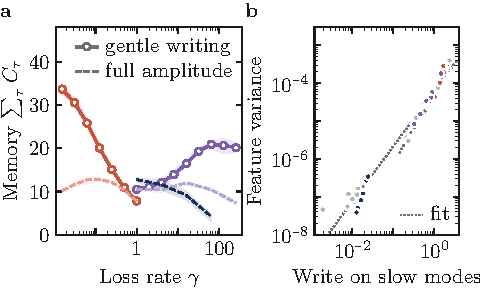
\includegraphics[width=\columnwidth]{figures/fig4_sampling.pdf}
\caption{\textbf{Measurement limits recoverable memory.}
\textbf{a}~Recoverable memory capacity at a budget of $10^9$ reservoir steps per output step: weak independent decay
with gentle writing recovers the most.
\textbf{b}~The signal, the mean variance of the exact features over the inputs, grows with the write strength, how
strongly an input changes the slow modes of the stationary state, for all channels at a matched decay-only lifetime.}
\label{fig:sampling}
\end{figure}
